\subsection{Módulo de radio}
El modelo de radio elegido ha sido el Sintonizador FM RDA5807M, mostrado en la \autoref{fig:2-3-Radio},  utilizado anteriormente en la asignatura de Sistemas Basados en Microprocesadores.

Dicho modelo se comunica con el microcontrolador mediante el protocolo \texttt{I2C}. El sintonizador cuenta con un decodificador MPX, salida de audio stereo y un rango de sintonización de 87 MHz a 108 MHz debido a nuestra situación geográfica.

En cuanto a la señal de audio de salida, hemos encontrado que presenta una componente continua de 1.65V y una amplitud de aproximadamente 1V. Debido a la conectividad que presenta el sintonizador, nos hemos encontrado el problema de que, al unirlo junto al resto del proyecto, cortocircuita la señal de masa analógica con la señal de masa virtual creada en nuestro circuito. Dicho problema se comentará en el \autoref{subsec:entre-dos-tierras}.

Por otra parte, necesita ser alimentado con una tensión entre 1.8V y 3.3V, soporta una corriente máxima de 10mA, cuenta con una relación señal-ruido típica de 55dB y presenta una distorsión armónica de audio total máxima del 0.2\%.

Todas las características de dicho sintonizador FM se han obtenido del datasheet ofrecido por el fabricante.
%REFERENCIA: DATASHEET RADIO

\begin{figure}[h]
    \centering
    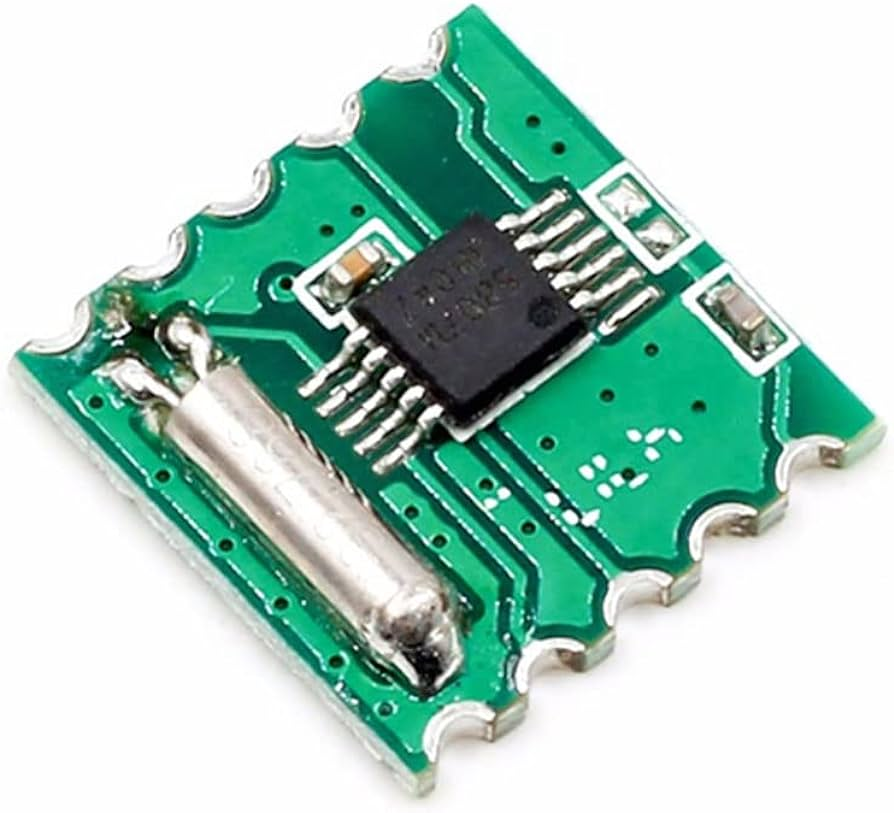
\includegraphics[width=0.3\textwidth]{images/2/2-3/Radio.jpg}
    \caption{Sintonizador FM RDA5807M}
    \label{fig:2-3-Radio}
\end{figure}